\documentclass[a4paper,12pt]{article}

\usepackage[utf8x]{inputenc}
\usepackage[T2A]{fontenc}
\usepackage[english, russian]{babel}

% Опционно, требует  apt-get install scalable-cyrfonts.*
% и удаления одной строчки в cyrtimes.sty
% Сточку не удалять!
% \usepackage{cyrtimes}

% Картнки и tikz
\usepackage{graphicx}
\usepackage{tikz}
\usetikzlibrary{snakes,arrows,shapes}


% Некоторая русификация.
\usepackage{misccorr}
\usepackage{indentfirst}
\renewcommand{\labelitemi}{\normalfont\bfseries{--}}

% Увы, поля придётся уменьшить из-за листингов.
\topmargin -1cm
\oddsidemargin -0.5cm
\evensidemargin -0.5cm
\textwidth 17cm
\textheight 24cm

\sloppy

% Оглавление в PDF
\usepackage[
bookmarks=true,
colorlinks=true, linkcolor=black, anchorcolor=black, citecolor=black, menucolor=black,filecolor=black, urlcolor=black,
unicode=true
]{hyperref}

% Для исходного кода в тексте
\newcommand{\Code}[1]{\texttt{#1}}


\title{Отчёт по лабораторной работе \\ <<Система доменных имён>>}
\author{Овчинников Владислав Александрович}

\begin{document}

\maketitle

\tableofcontents

\section{Настройка системы DNS}

BIND (Berkley Internet Name Domain) - открытая и наиболее распространенная реализация DNS-сервера, обеспечивающая выполнение преобразования DNS-имени в IP-адрес и наоборот. Исполняемый файл-демон сервера BIND называется named. 10 из 13 корневых серверов DNS работают на BIND, оставшиеся 3 работают на NSD.

\subsection{Топология сети}

Топология сети и использыемые IP-адреса показаны на рис.~\ref{fig:network}. Данная система не подключается к реальной сети и является самодостаточной. В состав системы входят:

1. Сеть \textbf{2.0.0.0/24}, имитирующая Интернет: 1) корневой DNS-сервер \textbf{dnsr} и два DNS-сервера (\textbf{dnsz1} и \textbf{dnsz2}), отвечающие за зоны имен; 2) два DNS-сервера (\textbf{dns1} и \textbf{dns2}), отвечающие за домены; 3) один NAT-маршрутизатор \textbf{r1}, являющийся также кеширующим DNS-сервером; 4) один почтовый сервер \textbf{mail2}, являющийся также кеширующим DNS-сервером.

2. Частная сеть \textbf{10.0.0.0/24}, доступная через NAT-маршрутизатор \textbf{r1}: 1) один почтовый сервер \textbf{mail1}; 2) один клиентский компьютер \textbf{pc1}, на котором установлен почтовый клиент.

Также была добавлена еще одна машина \textbf{dns3}, которая выполняет роль DNS-сервера по управлению доменным именем \textbf{nameserver.mynet}. Сделано это было с целью организации доступа к почтовому серверу, расположенному по данному адресу.

\begin{figure}
\centering
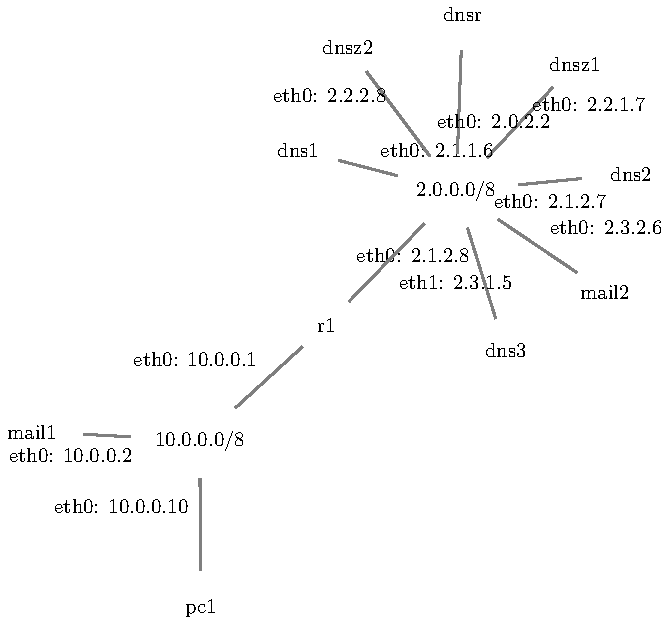
\includegraphics[width=\textwidth]{includes/network_gv.pdf}
\caption{Топология сети}
\label{fig:network}
\end{figure}

\subsection{Структура службы доменных имён}

Структура авторитетных серверов доменных имён показана на рис.~\ref{fig:dns}. 

Все файлы конфигурации на машинах ОС Debian находятся в каталоге \textbf{/etc/bind}.

При запуске сервер BIND считывает файл \textbf{named.conf}. В данном файле определяются прямая и обратная локальные зоны, их типы и файлы, в которых описываются dns-записи. Также в данном файле находится строчка, которая включает файл \textbf{named.conf.local}, в котором добавляются свои зоны.

Файл конфигурации \textbf{named.conf}, находящийся на корневом DNS-сервере, содержит:
\begin{verbatim}
options \{
    directory "/var/cache/bind";

    allow-recursion {"none";};

    recursion no;
\};

zone "localhost" \{
    type master;
    file "/etc/bind/db.local";
\};

zone "127.in-addr.arpa" \{
    type master;
    file "/etc/bind/db.127";
\};

zone "0.in-addr.arpa" \{
    type master;
    file "/etc/bind/db.0";
\};

zone "255.in-addr.arpa" \{
    type master;
    file "/etc/bind/db.255";
\};

include "/etc/bind/named.conf.local";
\end{verbatim}

\begin{figure}
\centering
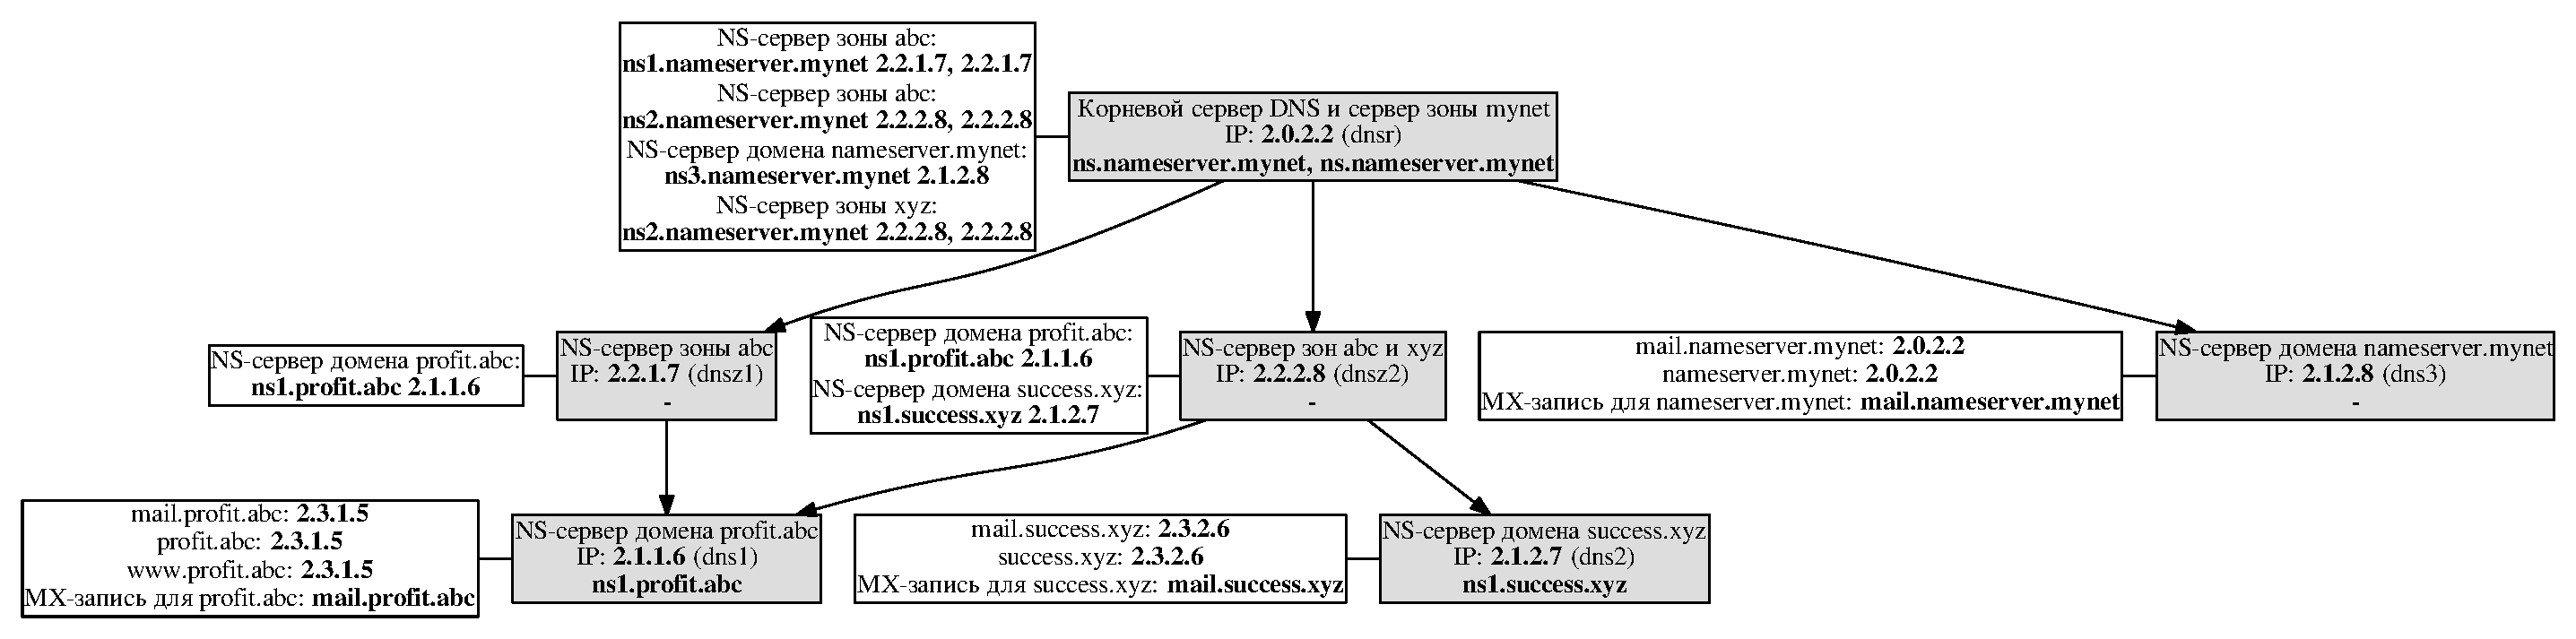
\includegraphics[width=\textwidth]{includes/dns_gv.pdf}
\caption{Структура службы доменных имён}
\label{fig:dns}
\end{figure}

Свои зоны добавляются в файл \textbf{named.conf.local}, который в данном случае содержит:
\begin{verbatim}
zone "." \{
    type master;
    file "/etc/bind/db.root";
    allow-query \{ any; \};
\};

zone "mynet" \{
    type master;
    file "/etc/bind/db.mynet";
    allow-query \{ any; \};
\};
\end{verbatim}

Стоит отметить, что корневые серверы DNS - это DNS-серверы, обеспечивающие работу корневой зоны DNS в сети Интернет. Корневые серверы DNS отвечают на запросы других DNS-серверов в ходе трансляции доменных имен в IP-адреса и позволяют получить список DNS-серверов для любого домена верхнего уровня.

В файле заданы 2 зоны ("." - корневая и "mynet" - служебная зона, в которой заведены записи для самих серверов имен, включая корневые). Первый параметр зоны - \textbf{type} (тип зоны), у обоих master (определяет зону, для которой данный сервер является первичным сервером). Также бывают \textbf{slave}, \textbf{hint} и \textbf{stub}.

Далее указан файл с информацией о данной зоне, имя у файлов может быть любое, но лучше всего задавать по типу \textbf{db.zonename}.

Параметр \textbf{allow-query} определяет хосты, которым разрешено выполнять запросы к DNS, \textbf{any} означает любые.

Содержимое файла \textbf{db.root}, который содержит информацию о корневой зоне ".":
\begin{verbatim}
$TTL    1D
.           IN SOA       ns.nameserver.mynet. admin.nameserver.mynet. (
                                       1
                                       4H
                                       1H
                                       1W
                                       1D )

                        IN NS   ns.nameserver.mynet.

abc.                    IN NS   ns1.nameserver.mynet.
abc.                    IN NS   ns2.nameserver.mynet.

xyz.                    IN NS   ns2.nameserver.mynet.

ns.nameserver.mynet.       IN A         2.0.2.2
ns2.nameserver.mynet.      IN A         2.2.2.8
ns1.nameserver.mynet.      IN A         2.2.1.7
\end{verbatim}

Авторитет сервера проистекает из того, что "вышестоящий" сервер сообщает о нем, как о сервере имен некоторой зоны. Авторитет корневого сервера заключается только в вере в него клиентов DNS.

Инструкция \$TTL задает время жизни зоны. Это значение определяет, как долго другие серверы будут кэшировать информацию об этой зоне.

Следующая запись - SOA (Start of Authority, начало авторитетности). Тут представлено краткое описание зоны - каково ее поведение и как серверам следует себя с ней вести. Цифры в SOA-записи управляют временем кеширования записей на кеширующих серверах. Два имени после слова SOA означает следующее: первое - основной NS-сервер (у зоны должен быть минимум один сервер имен), второе - почтовый адрес админа, где символ "@" заменен на первую по порядку точку. Запись после закрывающей скобки также относится к корневой зоне ".".

Записи с "IN NS" - это сервера имен, т.е. при запросе у этого сервера какой адрес, например, у \textbf{example.abc}, то он сначала посмотрит нет ли такого имени среди A-записей, и в случае неудачи выдаст все NS-сервера, ответственные за зону \textbf{abc.}, а именно \textbf{ns1.nameserver.mynet.} (\textbf{2.2.1.7}) и {ns2.nameserver.mynet.} (\textbf{2.2.2.8}).

Записи с "IN A" приводят к соответствию запрошенного домена IP-адресу.

Зона должна знать о всех нижестоящих NS-сервера, поэтому в этом файле прописана информация о зонах \textbf{abc.} и \textbf{xyz.}.

\subsection{Настройка MX-записей}

Для MX-записей настройка аналогична NS-серверам. В файле \textbf{db.success.xyz} на DNS-сервере \textbf{dns2}, отвечающем за доменное имя \textbf{success.xyz}, представлена настройка MX-записи:
\begin{verbatim}
$TTL    1D
success.xyz.           IN SOA       ns1.success.xyz. masha.success.xyz. (
                                       1
                                       1D
                                       1H
                                       1W
                                       1D )

                    IN NS        ns1.success.xyz.
success.xyz.        IN A         2.3.2.6
ns1.success.xyz.    IN A         2.1.2.7
success.xyz.        IN MX   10   mail.success.xyz.
mail.success.xyz.   IN A         2.3.2.6
\end{verbatim}

MX-запись задается с помощью "IN MX". Для одного домена может быть указано несколько почтовых серверов с разным предпочтением. Поэтой причине у MX-записи присутствует приоритет (в примере - 10), который указывает на то, какой сервер будет выбран первым. Также из примера видно, что почтовый сервер имеет доменное имя \textbf{mail.success.xyz}, которое является псевдонимом к адресу \textbf{2.3.2.6}.

\subsection{Прочие настройки}

Кеширующий DNS-сервер - обслуживает запросы клиентов (получает рекурсивный запрос, выполняет его с помощью нерекурсивных запросов к авторитетным серверам или передает рекурсивный запрос вышестоящему DNS-серверу).

Для кеширующего DNS-сервера используется программа PowerDNS. 

Кеширующие DNS-серверы в сети:
\begin{itemize}
\item mail2 - является одновременно и кеширующим DNS-сервером, и почтовым сервером;
\item r1 - является одновременно и кеширующим DNS-сервером, и NAT-маршрутизатором
\end{itemize}

Настраивается кеширующий DNS-сервер при помощи конфигурационного файла \textbf{/etc/powerdns/recursor.conf}, который содержит довольно обширное количество настроек, но интересует в данном случае только строчка:
\begin{verbatim}
hint-file=/etc/bind/db.root
\end{verbatim}

Данная строчка задает файл с указанными корневыми DNS-серверами, в данном случае \textbf{db.root} содержит для кеширующего DNS-сервера \textbf{r1}:
\begin{verbatim}
. 1D IN NS ns.nameserver.mynet
ns.nameserver.mynet. 1D IN A 2.0.2.2
\end{verbatim}

Все настройки почтового сервиса Exim4 хранятся в \textbf{/etc/exim4/update-exim4.conf.conf} на соответствующих машинах \textbf{mail1} и \textbf{mail2}.

Содержимое файла \textbf{update-exim4.conf.conf} на машине \textbf{mail1}:
\begin{verbatim}
dc_eximconfig_configtype='internet'
dc_other_hostnames='profit.abc'
dc_local_interfaces='0.0.0.0'
dc_readhost=''
dc_relay_domains=''
dc_minimaldns='false'
dc_relay_nets='10.0.0.0/8:127.0.0.1/8'
dc_smarthost=''
CFILEMODE='644'
dc_use_split_config='false'
dc_hide_mailname=''
dc_mailname_in_oh='true'
dc_localdelivery='mail_spool'
\end{verbatim} 

В данном файле \textbf{dc\_other\_hostnames} отвечает за имя домена почтового сервера, \textbf{dc\_relay\_nets} за список сетей, для которых открыт SMTP-сервер. В файле \textbf{/etc/mailname} также указывается доменное имя машины.

Развёрнутые SMTP-серверы и используемые ими кеширующие DNS-серверы.
\begin{itemize}
\item SMTP-сервер, развернутый на \textbf{mail1}, использует DNS-сервер, развернутый на \textbf{r1};
\item SMTP-сервер, развернутый на \textbf{mail2}, использует DNS-сервер, развернутый на этой же машине \textbf{mail2}
\end{itemize}


\section{Проверка настройки службы доменных имён}

Требовалось провести ряд экспериментов по проверке корректной настройки службы доменных имен (DNS).

\subsection{Проверка настройки записи типа A для домена profit.abc}

Поиск IP-адреса, соответствующего домену \textbf{profit.abc}, производилось при помощи последовательных запросов с помощью команды \textbf{dig}, начиная с корневого DNS-сервера, расположенного по адресу \textbf{2.0.2.2}. Все запросы выполнялись на машине \textbf{pc1}, которая представляет собой машину в частной сети с доступом в Интернет через NAT-маршрутизатор.

Первый запрос выполнялся при помощи команды \textbf{dig @2.0.2.2 profit.abc A}:
\begin{verbatim}
; <<>> DiG 9.5.0-P2 <<>> @2.0.2.2 profit.abc A
; (1 server found)
;; global options:  printcmd
;; Got answer:
;; ->>HEADER<<- opcode: QUERY, status: NOERROR, id: 53950
;; flags: qr rd; QUERY: 1, ANSWER: 0, AUTHORITY: 2, ADDITIONAL: 2
;; WARNING: recursion requested but not available

;; QUESTION SECTION:
;profit.abc.			IN	A

;; AUTHORITY SECTION:
abc.			86400	IN	NS	ns2.nameserver.mynet.
abc.			86400	IN	NS	ns1.nameserver.mynet.

;; ADDITIONAL SECTION:
ns1.nameserver.mynet.	86400	IN	A	2.2.1.7
ns2.nameserver.mynet.	86400	IN	A	2.2.2.8

;; Query time: 5 msec
;; SERVER: 2.0.2.2#53(2.0.2.2)
;; WHEN: Thu Dec 10 21:43:30 2020
;; MSG SIZE  rcvd: 112
\end{verbatim}

Первый вывод говорит о том, что записи о полном имени данного домена у корнего DNS-сервера нет, но есть информация о зоне \textbf{abc}, которая управляется двумя DNS-серверами (\textbf{ns1.nameserver.mynet} и \textbf{ns2.nameserver.mynet}). Для данных DNS-серверов также присутствуют записи на соответствие этих имен IP-адресам машин. Выбираем один из серверов по доступности.

Второй запрос выполнялся при помощи команды \textbf{dig @2.2.1.7 profit.abc A}:
\begin{verbatim}
; <<>> DiG 9.5.0-P2 <<>> @2.2.1.7 profit.abc A
; (1 server found)
;; global options:  printcmd
;; Got answer:
;; ->>HEADER<<- opcode: QUERY, status: NOERROR, id: 36664
;; flags: qr rd; QUERY: 1, ANSWER: 0, AUTHORITY: 1, ADDITIONAL: 1
;; WARNING: recursion requested but not available

;; QUESTION SECTION:
;profit.abc.			IN	A

;; AUTHORITY SECTION:
profit.abc.		86400	IN	NS	ns1.profit.abc.

;; ADDITIONAL SECTION:
ns1.profit.abc.		86400	IN	A	2.1.1.6

;; Query time: 26 msec
;; SERVER: 2.2.1.7#53(2.2.1.7)
;; WHEN: Thu Dec 10 21:53:50 2020
;; MSG SIZE  rcvd: 62
\end{verbatim}

Все еще не узнали об IP-адресе, который соответствует доменному имени \textbf{profit.abc}. Зато узнали, что данные домен управляется DNS-сервером \textbf{ns1.profit.abc}, расположенным по адресу \textbf{2.1.1.6}. Следовательно, необходимо выполнить еще один запрос.

Третий запрос выполнялся при помощи команды \textbf{dig @2.1.1.6 profit.abc A}:
\begin{verbatim}
; <<>> DiG 9.5.0-P2 <<>> @2.1.1.6 profit.abc A
; (1 server found)
;; global options:  printcmd
;; Got answer:
;; ->>HEADER<<- opcode: QUERY, status: NOERROR, id: 65263
;; flags: qr aa rd; QUERY: 1, ANSWER: 1, AUTHORITY: 1, ADDITIONAL: 1
;; WARNING: recursion requested but not available

;; QUESTION SECTION:
;profit.abc.			IN	A

;; ANSWER SECTION:
profit.abc.		86400	IN	A	2.3.1.5

;; AUTHORITY SECTION:
profit.abc.		86400	IN	NS	ns1.profit.abc.

;; ADDITIONAL SECTION:
ns1.profit.abc.		86400	IN	A	2.1.1.6

;; Query time: 7 msec
;; SERVER: 2.1.1.6#53(2.1.1.6)
;; WHEN: Thu Dec 10 21:56:24 2020
;; MSG SIZE  rcvd: 78
\end{verbatim}

Заключительный запрос говорит о том, что доменному имени с типом записи A соответствует IP-адрес \textbf{2.3.1.5}. Проверка на поиск соответствия выполнена успешно.

Также для проверки требовалось опросить кеширующий DNS-сервер, которым в данном случае выступает машина \textbf{r1}, являющаяся NAT-маршрутизатором. Подразумевается, что запрос будет отдан сразу без выполнения рекурсивного к авторитетным DNS-серверам.

Запрос к кеширующему DNS-серверу был выполнен при помощи команды \textbf{dig @10.0.0.1 profit.abc}:
\begin{verbatim}
; <<>> DiG 9.5.0-P2 <<>> @10.0.0.1 profit.abc
; (1 server found)
;; global options:  printcmd
;; Got answer:
;; ->>HEADER<<- opcode: QUERY, status: NOERROR, id: 44615
;; flags: qr rd ra; QUERY: 1, ANSWER: 1, AUTHORITY: 0, ADDITIONAL: 0

;; QUESTION SECTION:
;profit.abc.			IN	A

;; ANSWER SECTION:
profit.abc.		86322	IN	A	2.3.1.5

;; Query time: 3 msec
;; SERVER: 10.0.0.1#53(10.0.0.1)
;; WHEN: Thu Dec 10 22:03:55 2020
;; MSG SIZE  rcvd: 44
\end{verbatim}

Стоит отметить, что в это время на машинах \textbf{dns1}, \textbf{dnsz1} и \textbf{dnsr} был включен сниффер \textbf{tcpdump}, который не перехватил никакие сообщения от кеширующего DNS-сервера, что говорит, что он, действительно, отдал закешированную информацию о домене.

В случае же, если у DNS-сервера не будет сохраненных данных о домене в кеше, то сниффер перехватит следующие сообщения:
\begin{verbatim}
dnsr (корневой DNS-сервер)
22:15:44.254200 IP (tos 0x0, ttl 64, id 40316, offset 0, 
	flags [DF], proto UDP (17), length 56) 
	2.3.1.5.4809 > 2.2.1.7.53: [udp sum ok] 55666 A? profit.abc. (28)
22:15:44.254657 IP (tos 0x0, ttl 64, id 40316, offset 0, 
	flags [DF], proto UDP (17), length 56) 
	2.3.1.5.48364 > 2.1.1.6.53: [udp sum ok] 13783 A? profit.abc. (28)

dnsz (DNS-сервер, который управляет зоной abc)
22:15:44.252335 IP (tos 0x0, ttl 64, id 40316, offset 0, 
	flags [DF], proto UDP (17), length 56) 
	2.3.1.5.4809 > 2.2.1.7.53: [udp sum ok] 55666 A? profit.abc. (28)
22:15:44.252519 IP (tos 0x0, ttl 64, id 0, offset 0, 
	flags [DF], proto UDP (17), length 90) 
	2.2.1.7.53 > 2.3.1.5.4809: [udp sum ok] 55666- q: A? profit.abc. 0/1/1 ns: 
	profit.abc. NS ns1.profit.abc. ar: ns1.profit.abc. A 2.1.1.6 (62)
22:15:44.252790 IP (tos 0x0, ttl 64, id 40316, offset 0, 
	flags [DF], proto UDP (17), length 56) 
	2.3.1.5.48364 > 2.1.1.6.53: [udp sum ok] 13783 A? profit.abc. (28)

dns1 (DNS-сервер, который управляет непосредственно доменом profit.abc)
22:15:44.258084 IP (tos 0x0, ttl 64, id 40316, offset 0, 
	flags [DF], proto UDP (17), length 56) 
	2.3.1.5.4809 > 2.2.1.7.53: [udp sum ok] 55666 A? profit.abc. (28)
22:15:44.258546 IP (tos 0x0, ttl 64, id 40316, offset 0, 
	flags [DF], proto UDP (17), length 56) 
	2.3.1.5.48364 > 2.1.1.6.53: [udp sum ok] 13783 A? profit.abc. (28)
22:15:44.259350 IP (tos 0x0, ttl 64, id 0, offset 0, 
	flags [DF], proto UDP (17), length 106) 
	2.1.1.6.53 > 2.3.1.5.48364: [udp sum ok] 13783*- q: A? profit.abc. 1/1/1 
	profit.abc. A 2.3.1.5 ns: profit.abc. NS ns1.profit.abc. ar: 
	ns1.profit.abc. A 2.1.1.6 (78)
\end{verbatim}

Результат работы команды \textbf{ping profit.abc}:
\begin{verbatim}
PING profit.abc (2.3.1.5) 56(84) bytes of data.
64 bytes from 2.3.1.5: icmp_seq=1 ttl=64 time=0.143 ms
64 bytes from 2.3.1.5: icmp_seq=2 ttl=64 time=0.411 ms
64 bytes from 2.3.1.5: icmp_seq=3 ttl=64 time=0.294 ms
\end{verbatim}

\subsection{Проверка настройки записи типа NS для домена nameserver.mynet}

Также была выполнена проверка NS-записи для настроенного домена nameserver.mynet.

Первый вывод с помощью команды \textbf{dig @2.0.2.2 nameserver.mynet NS}:
\begin{verbatim}
; <<>> DiG 9.5.0-P2 <<>> @2.0.2.2 nameserver.mynet NS
; (1 server found)
;; global options:  printcmd
;; Got answer:
;; ->>HEADER<<- opcode: QUERY, status: NOERROR, id: 59960
;; flags: qr rd; QUERY: 1, ANSWER: 0, AUTHORITY: 1, ADDITIONAL: 1
;; WARNING: recursion requested but not available

;; QUESTION SECTION:
;nameserver.mynet.		IN	NS

;; AUTHORITY SECTION:
nameserver.mynet.	86400	IN	NS	ns3.nameserver.mynet.

;; ADDITIONAL SECTION:
ns3.nameserver.mynet.	86400	IN	A	2.1.2.8

;; Query time: 3 msec
;; SERVER: 2.0.2.2#53(2.0.2.2)
;; WHEN: Thu Dec 10 22:23:46 2020
;; MSG SIZE  rcvd: 68
\end{verbatim}

Второй вывод с помощью команды \textbf{dig @2.1.2.8 nameserver.mynet NS}:
\begin{verbatim}
; <<>> DiG 9.5.0-P2 <<>> @2.1.2.8 nameserver.mynet NS
; (1 server found)
;; global options:  printcmd
;; Got answer:
;; ->>HEADER<<- opcode: QUERY, status: NOERROR, id: 63742
;; flags: qr aa rd; QUERY: 1, ANSWER: 1, AUTHORITY: 0, ADDITIONAL: 0
;; WARNING: recursion requested but not available

;; QUESTION SECTION:
;nameserver.mynet.		IN	NS

;; ANSWER SECTION:
nameserver.mynet.	86400	IN	NS	ns3.nameserver.mynet.

;; Query time: 14 msec
;; SERVER: 2.1.2.8#53(2.1.2.8)
;; WHEN: Thu Dec 10 22:24:38 2020
;; MSG SIZE  rcvd: 52
\end{verbatim}

Была проведена проверка кеширующего DNS-сервера c помощью команды \textbf{dig @10.0.0.1 nameserver.mynet NS}:
\begin{verbatim}
; <<>> DiG 9.5.0-P2 <<>> @10.0.0.1 nameserver.mynet NS
; (1 server found)
;; global options:  printcmd
;; Got answer:
;; ->>HEADER<<- opcode: QUERY, status: NOERROR, id: 50277
;; flags: qr rd ra; QUERY: 1, ANSWER: 1, AUTHORITY: 0, ADDITIONAL: 1

;; QUESTION SECTION:
;nameserver.mynet.		IN	NS

;; ANSWER SECTION:
nameserver.mynet.	83040	IN	NS	ns3.nameserver.mynet.

;; ADDITIONAL SECTION:
ns3.nameserver.mynet.	83040	IN	A	2.1.2.8

;; Query time: 1 msec
;; SERVER: 10.0.0.1#53(10.0.0.1)
;; WHEN: Thu Dec 10 22:27:54 2020
;; MSG SIZE  rcvd: 68
\end{verbatim}

Вывод команды \textbf{ping nameserver.mynet}:
\begin{verbatim}
PING nameserver.mynet (2.0.2.2) 56(84) bytes of data.
64 bytes from 2.0.2.2: icmp_seq=1 ttl=63 time=10.6 ms
64 bytes from 2.0.2.2: icmp_seq=2 ttl=63 time=0.644 ms
64 bytes from 2.0.2.2: icmp_seq=3 ttl=63 time=0.592 ms
64 bytes from 2.0.2.2: icmp_seq=4 ttl=63 time=0.679 ms
\end{verbatim}

Все эксперименты по проверке NS-записи \textbf{nameserver.mynet} были проведены успешно.

\section{Проверка работы почтовой системы}

\subsection{Проверка MX-записи для домена \textbf{mail.success.xyz}}

С узла \textbf{ps1} было отправлено письмо на локальный SMTP-сервер для адресата с адресом \textbf{admin@success.xyz}.

Лог, собранный с помощью \textbf{tcpdump}:
\begin{verbatim}
IP 2.3.1.5.54606 > 2.3.2.6.25: S 1465056111:1465056111(0) win 5840 
		<mss 1460,sackOK,timestamp 383572 0,nop,wscale 1>
IP 2.3.2.6.25 > 2.3.1.5.54606: S 1460753955:1460753955(0) ack 1465056112 win 5792 
		<mss 1460,sackOK,timestamp 383573 383572,nop,wscale 1>
IP 2.3.1.5.54606 > 2.3.2.6.25: . ack 1 win 2920 
		<nop,nop,timestamp 383572 383573>
IP 2.3.2.6.53888 > 2.3.1.5.113: S 1459683900:1459683900(0) win 5840 
		<mss 1460,sackOK,timestamp 383573 0,nop,wscale 1>
IP 2.3.1.5.113 > 2.3.2.6.53888: R 0:0(0) ack 1459683901 win 0
IP 2.3.2.6.25 > 2.3.1.5.54606: P 1:60(59) ack 1 win 2896 
		<nop,nop,timestamp 383575 383572>
IP 2.3.1.5.54606 > 2.3.2.6.25: . ack 60 win 2920 
		<nop,nop,timestamp 383575 383575>
IP 2.3.1.5.54606 > 2.3.2.6.25: P 1:14(13) ack 60 win 2920 
		<nop,nop,timestamp 383871 383575>
IP 2.3.2.6.25 > 2.3.1.5.54606: . ack 14 win 2896 
		<nop,nop,timestamp 383870 383871>
IP 2.3.2.6.25 > 2.3.1.5.54606: P 60:94(34) ack 14 win 2896 
		<nop,nop,timestamp 383870 383871>
IP 2.3.1.5.54606 > 2.3.2.6.25: . ack 94 win 2920 
		<nop,nop,timestamp 383871 383870>
IP 2.3.1.5.54606 > 2.3.2.6.25: P 57:99(42) ack 120 win 2920 
		<nop,nop,timestamp 397274 392457>
IP 2.3.2.6.25 > 2.3.1.5.54606: P 120:128(8) ack 99 win 2896 
		<nop,nop,timestamp 397273 397274>
IP 2.3.1.5.54606 > 2.3.2.6.25: . ack 128 win 2920 
		<nop,nop,timestamp 397274 397273>
IP 2.3.1.5.54606 > 2.3.2.6.25: P 99:128(29) ack 128 win 2920 
		<nop,nop,timestamp 402021 397273>
IP 2.3.2.6.25 > 2.3.1.5.54606: P 128:142(14) ack 128 win 2896 
		<nop,nop,timestamp 402020 402021>
IP 2.3.1.5.54606 > 2.3.2.6.25: . ack 142 win 2920 
		<nop,nop,timestamp 402021 402020>
IP 2.3.1.5.54606 > 2.3.2.6.25: P 128:134(6) ack 142 win 2920 
		<nop,nop,timestamp 406182 402020>
IP 2.3.2.6.25 > 2.3.1.5.54606: P 142:198(56) ack 134 win 2896 
		<nop,nop,timestamp 406181 406182>
IP 2.3.1.5.54606 > 2.3.2.6.25: . ack 198 win 2920 
		<nop,nop,timestamp 406182 406181>
IP 2.3.1.5.54606 > 2.3.2.6.25: P 134:149(15) ack 198 win 2920 
		<nop,nop,timestamp 409666 406181>
IP 2.3.2.6.25 > 2.3.1.5.54606: . ack 149 win 2896 
		<nop,nop,timestamp 409669 409666>
IP 2.3.1.5.54606 > 2.3.2.6.25: P 149:151(2) ack 198 win 2920 
		<nop,nop,timestamp 411778 409669>
IP 2.3.2.6.25 > 2.3.1.5.54606: . ack 151 win 2896 
		<nop,nop,timestamp 411777 411778>
IP 2.3.1.5.54606 > 2.3.2.6.25: P 151:166(15) ack 198 win 2920 
		<nop,nop,timestamp 413219 411777>
IP 2.3.2.6.25 > 2.3.1.5.54606: . ack 166 win 2896 
		<nop,nop,timestamp 413218 413219>
IP 2.3.1.5.54606 > 2.3.2.6.25: P 166:169(3) ack 198 win 2920 
		<nop,nop,timestamp 413299 413218>
IP 2.3.2.6.25 > 2.3.1.5.54606: . ack 169 win 2896 
		<nop,nop,timestamp 413298 413299>
IP 2.3.2.6.25 > 2.3.1.5.54606: P 198:226(28) ack 169 win 2896 
		<nop,nop,timestamp 413298 413299>
IP 2.3.1.5.54606 > 2.3.2.6.25: . ack 226 win 2920 
		<nop,nop,timestamp 413299 413298>
\end{verbatim}

Процесс общения с SMTP-сервером:
\begin{verbatim}
220 mail2 ESMTP Exim 4.69 Thu, 10 Dec 2020 22:40:10 +0000
HELO client
250 mail2 Hello client [2.3.1.5]
MAIL from:<vladovchinnikov950@gmail.com>
500 unrecognized command
MAIL from:<vladovchinnikov950@gmail.com>
250 OK
RCPT to:<admin@success.xyz>
250 Accepted
DATA
354 Enter message, ending with "." on a line by itself
Subject: Test

Hello, world!
.
250 OK id=1knUfE-0000Mf-L9
\end{verbatim}

На машине \textbf{mail2} с доменным именем \textbf{success.xyz} появилось доставленное письмо:
\begin{verbatim}
cat /var/mail/admin

From vladovchinnikov950@gmail.com Thu Dec 10 22:45:07 2020
Return-path: <vladovchinnikov950@gmail.com>
Envelope-to: admin@success.xyz
Delivery-date: Thu, 10 Dec 2020 22:45:07 +0000
Received: from [2.3.1.5] (helo=client)
	by mail2 with smtp (Exim 4.69)
	(envelope-from <vladovchinnikov950@gmail.com>)
	id 1knUfE-0000Mf-L9
	for admin@success.xyz; Thu, 10 Dec 2020 22:45:07 +0000
Subject: Test

Hello, world!
\end{verbatim}

Таким образом, доменная запись типа MX для домена \textbf{success.xyz} настроена верно.

\subsection{Проверка MX-записи для домена \textbf{profit.abc}}

С узла \textbf{ps1} было отправлено письмо на локальный SMTP-сервер для адресата с адресом \textbf{admin@profit.abc}.

Лог, собранный с помощью \textbf{tcpdump}:
\begin{verbatim}
IP 10.0.0.1.56057 > 10.0.0.2.25: S 1207826151:1207826151(0) win 5840 
		<mss 1460,sackOK,timestamp 600971 0,nop,wscale 1>
IP 10.0.0.2.25 > 10.0.0.1.56057: S 1206206930:1206206930(0) ack 1207826152 win 5792 
		<mss 1460,sackOK,timestamp 600886 600971,nop,wscale 1>
IP 10.0.0.1.56057 > 10.0.0.2.25: . ack 1 win 2920 
		<nop,nop,timestamp 600971 600886>
IP 10.0.0.2.47287 > 10.0.0.1.113: S 1207725875:1207725875(0) win 5840 
		<mss 1460,sackOK,timestamp 600886 0,nop,wscale 1>
IP 10.0.0.1.113 > 10.0.0.2.47287: R 0:0(0) ack 1207725876 win 0
IP 10.0.0.2.25 > 10.0.0.1.56057: P 1:60(59) ack 1 win 2896 
		<nop,nop,timestamp 600886 600971>
IP 10.0.0.1.56057 > 10.0.0.2.25: . ack 60 win 2920 
		<nop,nop,timestamp 600975 600886>
IP 10.0.0.1.56057 > 10.0.0.2.25: P 1:14(13) ack 60 win 2920 
		<nop,nop,timestamp 601656 600886>
IP 10.0.0.2.25 > 10.0.0.1.56057: . ack 14 win 2896 
		<nop,nop,timestamp 601568 601656>
IP 10.0.0.2.25 > 10.0.0.1.56057: P 60:95(35) ack 14 win 2896 
		<nop,nop,timestamp 601568 601656>
IP 10.0.0.1.56057 > 10.0.0.2.25: . ack 95 win 2920 
		<nop,nop,timestamp 601656 601568>
IP 10.0.0.1.56057 > 10.0.0.2.25: P 14:56(42) ack 95 win 2920 
		<nop,nop,timestamp 603198 601568>
IP 10.0.0.2.25 > 10.0.0.1.56057: P 95:103(8) ack 56 win 2896 
		<nop,nop,timestamp 603110 603198>
IP 10.0.0.1.56057 > 10.0.0.2.25: . ack 103 win 2920 
		<nop,nop,timestamp 603198 603110>
IP 10.0.0.1.56057 > 10.0.0.2.25: P 56:84(28) ack 103 win 2920 
		<nop,nop,timestamp 604325 603110>
IP 10.0.0.2.25 > 10.0.0.1.56057: P 103:117(14) ack 84 win 2896 
		<nop,nop,timestamp 604238 604325>
IP 10.0.0.1.56057 > 10.0.0.2.25: . ack 117 win 2920 
		<nop,nop,timestamp 604325 604238>
IP 10.0.0.1.56057 > 10.0.0.2.25: P 84:90(6) ack 117 win 2920 
		<nop,nop,timestamp 604580 604238>
IP 10.0.0.2.25 > 10.0.0.1.56057: P 117:173(56) ack 90 win 2896 
		<nop,nop,timestamp 604492 604580>
IP 10.0.0.1.56057 > 10.0.0.2.25: . ack 173 win 2920 
		<nop,nop,timestamp 604580 604492>
IP 10.0.0.1.56057 > 10.0.0.2.25: P 90:105(15) ack 173 win 2920 
		<nop,nop,timestamp 605305 604492>
IP 10.0.0.2.25 > 10.0.0.1.56057: . ack 105 win 2896 
		<nop,nop,timestamp 605221 605305>
IP 10.0.0.1.56057 > 10.0.0.2.25: P 105:107(2) ack 173 win 2920 
		<nop,nop,timestamp 605388 605221>
IP 10.0.0.2.25 > 10.0.0.1.56057: . ack 107 win 2896 
		<nop,nop,timestamp 605300 605388>
IP 10.0.0.1.56057 > 10.0.0.2.25: P 107:122(15) ack 173 win 2920 
		<nop,nop,timestamp 605813 605300>
IP 10.0.0.2.25 > 10.0.0.1.56057: . ack 122 win 2896 
		<nop,nop,timestamp 605725 605813>
IP 10.0.0.1.56057 > 10.0.0.2.25: P 122:125(3) ack 173 win 2920 
		<nop,nop,timestamp 605934 605725>
IP 10.0.0.2.25 > 10.0.0.1.56057: . ack 125 win 2896 
		<nop,nop,timestamp 605846 605934>
IP 10.0.0.2.25 > 10.0.0.1.56057: P 173:201(28) ack 125 win 2896 
		<nop,nop,timestamp 605846 605934>
IP 10.0.0.1.56057 > 10.0.0.2.25: . ack 201 win 2920 
		<nop,nop,timestamp 605934 605846>
\end{verbatim}

Процесс общения с SMTP-сервером:
\begin{verbatim}
220 mail1 ESMTP Exim 4.69 Thu, 10 Dec 2020 23:14:58 +0000
^C^[[A^]
telnet> q
Connection closed.
pc1:~# telnet profit.abc 25
Trying 2.3.1.5...
Connected to profit.abc.
Escape character is '^]'.
220 mail1 ESMTP Exim 4.69 Thu, 10 Dec 2020 23:16:24 +0000
HELO client
250 mail1 Hello client [10.0.0.1]
MAIL from:<vladovchinnikov950@gmail.com>
250 OK
RCPT to:<admin@profit.abc>
250 Accepted
DATA
354 Enter message, ending with "." on a line by itself
Subject: Test   

Hello, world.
.
250 OK id=1knVBE-0000VN-Kt
\end{verbatim}

На машине \textbf{mail1} с доменным именем \textbf{profit.abc} появилось доставленное письмо:
\begin{verbatim}
cat /var/mail/admin

From vladovchinnikov950@gmail.com Thu Dec 10 23:17:14 2020
Return-path: <vladovchinnikov950@gmail.com>
Envelope-to: admin@profit.abc
Delivery-date: Thu, 10 Dec 2020 23:17:14 +0000
Received: from [10.0.0.1] (helo=client)
	by mail1 with smtp (Exim 4.69)
	(envelope-from <vladovchinnikov950@gmail.com>)
	id 1knVBE-0000VN-Kt
	for admin@profit.abc; Thu, 10 Dec 2020 23:17:14 +0000
Subject: Test
Message-Id: <E1knVBE-0000VN-Kt@mail1>
From: vladovchinnikov950@gmail.com
Date: Thu, 10 Dec 2020 23:17:08 +0000

Hello, world.
\end{verbatim}

Таким образом, доменная запись типа MX для домена \textbf{profit.abc} настроена верно.

\subsection{Проверка MX-записи для домена \textbf{nameserver.mynet}}

С узла \textbf{ps1} было отправлено письмо на локальный SMTP-сервер для адресата с адресом \textbf{admin@nameserver.mynet}.

Лог, собранный с помощью \textbf{tcpdump}:
\begin{verbatim}
IP 2.3.1.5.39202 > 2.0.2.2.25: S 2930723193:2930723193(0) win 5840 
		<mss 1460,sackOK,timestamp 639376 0,nop,wscale 1>
IP 2.0.2.2.25 > 2.3.1.5.39202: S 2932624253:2932624253(0) ack 2930723194 win 5792 
		<mss 1460,sackOK,timestamp 639405 639376,nop,wscale 1>
IP 2.3.1.5.39202 > 2.0.2.2.25: . ack 1 win 2920 
		<nop,nop,timestamp 639377 639405>
IP 2.0.2.2.55604 > 2.3.1.5.113: S 2924283154:2924283154(0) win 5840 
		<mss 1460,sackOK,timestamp 639405 0,nop,wscale 1>
IP 2.3.1.5.113 > 2.0.2.2.55604: R 0:0(0) ack 2924283155 win 0
IP 2.0.2.2.25 > 2.3.1.5.39202: P 1:59(58) ack 1 win 2896 
		<nop,nop,timestamp 639405 639377>
IP 2.3.1.5.39202 > 2.0.2.2.25: . ack 59 win 2920 
		<nop,nop,timestamp 639378 639405>
IP 2.3.1.5.39202 > 2.0.2.2.25: P 1:14(13) ack 59 win 2920 
		<nop,nop,timestamp 639720 639405>
IP 2.0.2.2.25 > 2.3.1.5.39202: . ack 14 win 2896 
		<nop,nop,timestamp 639747 639720>
IP 2.0.2.2.25 > 2.3.1.5.39202: P 59:92(33) ack 14 win 2896 
		<nop,nop,timestamp 639747 639720>
IP 2.3.1.5.39202 > 2.0.2.2.25: . ack 92 win 2920 
		<nop,nop,timestamp 639720 639747>
IP 2.3.1.5.39202 > 2.0.2.2.25: P 14:56(42) ack 92 win 2920 
		<nop,nop,timestamp 641018 639747>
IP 2.0.2.2.25 > 2.3.1.5.39202: P 92:100(8) ack 56 win 2896 
		<nop,nop,timestamp 641046 641018>
IP 2.3.1.5.39202 > 2.0.2.2.25: . ack 100 win 2920 
		<nop,nop,timestamp 641018 641046>
IP 2.3.1.5.39202 > 2.0.2.2.25: P 56:90(34) ack 100 win 2920 
		<nop,nop,timestamp 642199 641046>
IP 2.0.2.2.25 > 2.3.1.5.39202: P 100:114(14) ack 90 win 2896 
		<nop,nop,timestamp 642227 642199>
IP 2.3.1.5.39202 > 2.0.2.2.25: . ack 114 win 2920 
		<nop,nop,timestamp 642199 642227>
IP 2.3.1.5.39202 > 2.0.2.2.25: P 90:96(6) ack 114 win 2920 
		<nop,nop,timestamp 642595 642227>
IP 2.0.2.2.25 > 2.3.1.5.39202: P 114:170(56) ack 96 win 2896 
		<nop,nop,timestamp 642623 642595>
IP 2.3.1.5.39202 > 2.0.2.2.25: . ack 170 win 2920 
		<nop,nop,timestamp 642595 642623>
IP 2.3.1.5.39202 > 2.0.2.2.25: P 96:111(15) ack 170 win 2920 
		<nop,nop,timestamp 643142 642623>
IP 2.0.2.2.25 > 2.3.1.5.39202: . ack 111 win 2896 
		<nop,nop,timestamp 643174 643142>
IP 2.3.1.5.39202 > 2.0.2.2.25: P 111:113(2) ack 170 win 2920 
		<nop,nop,timestamp 643169 643174>
IP 2.0.2.2.25 > 2.3.1.5.39202: . ack 113 win 2896 
		<nop,nop,timestamp 643196 643169>
IP 2.3.1.5.39202 > 2.0.2.2.25: P 113:127(14) ack 170 win 2920 
		<nop,nop,timestamp 643661 643196>
IP 2.0.2.2.25 > 2.3.1.5.39202: . ack 127 win 2896 
		<nop,nop,timestamp 643688 643661>
IP 2.3.1.5.39202 > 2.0.2.2.25: P 127:130(3) ack 170 win 2920 
		<nop,nop,timestamp 643735 643688>
IP 2.0.2.2.25 > 2.3.1.5.39202: . ack 130 win 2896 
		<nop,nop,timestamp 643762 643735>
IP 2.0.2.2.25 > 2.3.1.5.39202: P 170:198(28) ack 130 win 2896 
		<nop,nop,timestamp 643762 643735>
IP 2.3.1.5.39202 > 2.0.2.2.25: . ack 198 win 2920 
		<nop,nop,timestamp 643735 643762>
\end{verbatim}

Процесс общения с SMTP-сервером:
\begin{verbatim}
220 dnsr ESMTP Exim 4.69 Thu, 10 Dec 2020 23:22:48 +0000
HELO client
250 dnsr Hello client [2.3.1.5]
MAIL from:<vladovchinnikov950@gmail.com>
250 OK
RCPT to:<admin@nameserver.mynet>
250 Accepted
DATA
354 Enter message, ending with "." on a line by itself
Subject: Test 

Hello, test.
.
250 OK id=1knVHM-0000Eh-Us
\end{verbatim}

На машине \textbf{dnsr} с доменным именем \textbf{nameserver.mynet} появилось доставленное письмо:
\begin{verbatim}
cat /var/mail/admin

From vladovchinnikov950@gmail.com Thu Dec 10 23:23:32 2020
Return-path: <vladovchinnikov950@gmail.com>
Envelope-to: admin@nameserver.mynet
Delivery-date: Thu, 10 Dec 2020 23:23:32 +0000
Received: from [2.3.1.5] (helo=client)
	by dnsr with smtp (Exim 4.69)
	(envelope-from <vladovchinnikov950@gmail.com>)
	id 1knVHM-0000Eh-Us
	for admin@nameserver.mynet; Thu, 10 Dec 2020 23:23:32 +0000
Subject: Test
Message-Id: <E1knVHM-0000Eh-Us@dnsr>
From: vladovchinnikov950@gmail.com
Date: Thu, 10 Dec 2020 23:23:26 +0000

Hello, test.
\end{verbatim}

Таким образом, доменная запись типа MX для домена \textbf{nameserver.mynet} настроена верно.

\end{document}
